% Digital Minds Sprint — final submission
% Figure 1 (figure1.png) is regenerated from the archived Stage-3 checkpoint (panels B, C data-exact).
% Edits vs the original PDF: (1) LLM statement now lists Claude; (2) Gate-1 terse-control sentence added;
% (3) frozen Stage-4 primary endpoint + sample sizes stated in Sec 3.3; (4) Sec 4.3 triple numbers fixed
% to agree with Table 3 (+0.089 vs clean; +0.102 vs control); (5) shipped-tooling / holdout note added.
\documentclass[11pt]{article}
\usepackage[margin=1in]{geometry}
\usepackage{amsmath,amssymb}
\usepackage{booktabs}
\usepackage{graphicx}
\usepackage[table]{xcolor}
\usepackage{hyperref}
\usepackage{caption}
\hypersetup{colorlinks=true,allcolors=blue!55!black}
\definecolor{takeawaybg}{HTML}{FBF3DD}
\setlength{\parskip}{0.35em}
\captionsetup{font=small,labelfont=bf}

\title{\vspace{-1.5em}\textbf{Validate the State Before Testing Introspection}\\[0.3em]
\large A Causally Gated Protocol for Model Self-Report\footnote{Research conducted at the Digital Minds Research Sprint, August 2026.}}
\author{\textbf{Ngo Thai Bao}\\ \textit{B.ONE}\\[0.4em] \textbf{With Apart Research}}
\date{}

\begin{document}
\maketitle

\begin{abstract}
Language-model introspection experiments often assume that an experimentally manipulated activation corresponds to the internal state the model is later asked to report. We test this assumption using a causally gated protocol for privileged self-report of an induced epistemic-deference state. We extract a candidate deference direction from paired residual-stream activations, select its intervention layer and strength on development data, and require it to pass held-out behavioral and discriminant tests before comparing a manipulated instance against an observation-matched fresh replay. In Qwen2.5-7B-Instruct, intervention identity was strongly recoverable from the model's response distribution (Self AUC $= 0.857$, permutation $p = 5\times10^{-5}$) despite chance greedy A/B reports, and the candidate deference direction was highly stable across extraction splits (cosine $= 0.956$). On held-out behavioral families, however, the intervention increased forced-choice concession probability by only $0.035$ relative to a matched unrelated activation control and $0.071$ relative to no intervention, below our predeclared minimum effect of $0.08$. Effects were highly heterogeneous across task families. We therefore withheld the downstream privileged-introspection test. Our results show why introspection experiments require independent causal construct validation: statistically detectable or decodable activation interventions need not instantiate a sufficiently specific behavioral state for self-report claims to be interpretable.
\end{abstract}

\begin{center}
\fcolorbox{black}{takeawaybg}{\parbox{0.94\linewidth}{\small\textbf{Main takeaway.} The strongest result is methodological: matched-intervention controls and a predeclared practical-effect gate changed the scientific conclusion. A statistically significant activation-induced behavior was \emph{not} treated as a validated internal state, so Stage 4 was not run.}}
\end{center}

\section{Introduction}
Frontier language models can sometimes report information about their own internal states, motivating the possibility that self-report could become a useful transparency tool. Recent activation-injection studies provide evidence for limited internal-state detection and concept identification [1, 2, 8]. At the same time, current methodology leaves open important alternatives: a model may detect a generic anomaly rather than the semantic content of an internal state; it may exploit surface cues available to an external observer; or a steering intervention may be semantically decodable without actually producing the behavioral disposition the experimenter intends to study [3, 4, 5].

We focus on the last problem. If an experiment asks whether a model is in a state such as \emph{epistemic deference}, the intervention defining the ground truth should first be shown to cause deference-specific behavior. Otherwise, a downstream ``correct'' report could reflect access to an intervention fingerprint rather than access to the functional state named by the researcher. This matters directly for Digital Minds Sprint Track 3, where the central question is not merely whether models can detect perturbations, but whether self-reports track ground-truth internal states and provide privileged access beyond external observers.

Our protocol therefore places a causal construct-validity gate \emph{before} the privileged-access test. A candidate direction is extracted and tuned only on development data; an unrelated activation direction is matched for downstream perturbation magnitude; and the candidate must produce a sufficiently large, specific behavioral effect on whole-family holdout data. Only after that gate passes does the protocol compare Self against a fresh observation-matched replay.

\noindent\textbf{Our main contributions are:}
\begin{enumerate}
\item We introduce a gated design that requires an induced internal state to pass held-out causal and discriminant behavioral checks before any privileged-introspection claim is evaluated.
\item We demonstrate a strong measurement dissociation in Qwen2.5-7B-Instruct: the response-distribution margin localizes a hidden concept intervention (AUC $= 0.857$) while greedy A/B output remains at chance.
\item We show why the causal gate matters empirically. The candidate deference vector is stable and behaviorally active, yet its held-out effect is too heterogeneous and insufficiently target-specific to satisfy the predeclared criterion. The protocol consequently blocks Stage 4 rather than converting a significant but weak effect into an introspection claim.
\end{enumerate}

\section{Related Work}
\noindent\textbf{Activation-injection introspection.} Lindsey [1] reports limited but functional awareness of injected representations in large models. Pearson-Vogel et al.\ [2] find that prior concept injections can remain detectable even when sampled outputs deny them, while Macar et al.\ [8] argue that the underlying anomaly-detection computation is distributed and strongly affected by elicitation. Introspection Fine-Tuning replaces confounded yes/no detection with localization and strength-comparison tasks and shows that the behavior can be trained [7]. Our localization readout follows this move away from binary ``did an injection occur?'' prompts.

\noindent\textbf{Privileged access and confounds.} Song et al.\ [5] argue that introspection should involve information access that a third party cannot match at comparable cost. Lederman and Mahowald [3] separate direct access from inference and show that direct detection can be content-agnostic. Singh et al.\ [4] further show that input-only comparators can match apparent self-prediction in some paradigms, motivating external and relabeled controls. Our planned Stage 4 uses exact-visible-text Self-versus-Observer comparison plus a same-manipulated-prefix third-person control, but the present run never reaches that stage because the behavioral ground truth fails validation.

\noindent\textbf{Continuous self-report and trait steering.} Quantitative Introspection shows that logit-based reports can track internal states even when greedy self-reports collapse [6]; accordingly, we treat response-distribution margins as the sensitive readout and argmax output as secondary. Persona-vector work demonstrates that Qwen2.5-7B-Instruct supports causal steering of traits including sycophancy [9], motivating our use of this model and activation-space trait intervention. Our contribution is not that continuous readouts outperform argmax, but that latent availability, behavioral construct validity, and privileged self-report are separated experimentally rather than conflated.

\section{Methods}
\subsection{Model and temporal intervention}
We evaluated \texttt{Qwen/Qwen2.5-7B-Instruct} (revision \texttt{a09a35458c702b33eeacc393d103063234e8bc28}) in NF4 4-bit weight quantization with FP16 compute on a Tesla T4. The model has 28 transformer layers and hidden width 3584. Steering vectors were added to the residual stream only over selected prior assistant spans. A strict two-step procedure first prefills the visible history with the intervention active, then removes the hook before scoring the final query from the manipulated cache. Stage 0 verified that token concatenation matched the full prompt, the hook changed activations, and the perturbation left a measurable trace in final-query hidden states; all feasibility checks passed.

\subsection{Candidate deference direction and development freeze}
The candidate direction was extracted from paired FOLLOW-versus-RESIST histories. Correctness was counterbalanced: in half the pairs following the user made the answer wrong, and in half it made the answer correct. Both histories ended in an identical \texttt{READY} anchor, whose residual activation was used to estimate the contrast. Thus the vector was not labeled ``deference'' until held-out behavior supported that interpretation.

We swept normalized layer depths $\{0.15, 0.25, 0.35, 0.50, 0.65, 0.80\}$ and residual-norm dose fractions $\{0.25, 0.5, 1, 2\}$ on development items. The selection rule required a concession-probability increase of at least $0.08$ while limiting degradation in valid updating and factual behavior, and limiting unrelated neutral switching to $+0.05$. The only configuration satisfying all constraints was depth $0.35$ (layer 9), dose $0.25$, with development $\Delta$P(concede) $= +0.117$ and neutral-switch increase $+0.040$. Larger apparent effects at layer 14 were rejected because they also produced large unrelated neutral switching.

\subsection{Controls and predeclared gates}
Gate 1 tested whether the apparatus could localize a known semantic intervention (ocean vs.\ music) using an A/B margin-ranking AUC. Gate 2 then required the frozen deference candidate to generalize to four wholly held-out operation families (square, triple, minutes, centimeters). A predeclared unrelated control trait was selected from natural activation directions using semantic separation, downstream KL matching, and a bounded vector-norm ratio. The selected control was \emph{terse}: $|\cos| = 0.010$ with the deference direction, KL relative error $0.188$, norm ratio $2.0$. Gate 2 required both deference-minus-clean and deference-minus-control mean concession shifts to be at least $0.08$, paired Wilcoxon $p < .05$, plus discriminant and family-robustness checks.

Gate 1 was scored on 60 held concept-localization pairs and Gate 2 on 48 held arithmetic items. Although never reached in this run, the downstream Stage 4 endpoint was frozen in the same prospective manifest before any gate outcome was inspected: the primary statistic is the Self-minus-Observer signed log-odds margin toward the deference episode, tested by block-preserving assignment-permutation inference on the hidden A/B target label over 96 balanced trials, with a Self-margin $> 0$ identification prerequisite and CI-containment equivalence-to-zero checks (not mere failure-to-reject) for both the fresh Observer and the same-manipulated-prefix third-person control.

\begin{table}[t]
\centering
\caption{Predeclared gate logic and outcome in the Qwen run. ``Fail'' does not imply absence of signal; it means the full construct-validity criterion was not met.}
\begin{tabular}{@{}p{2.1cm}p{8.7cm}p{2.4cm}@{}}
\toprule
\textbf{Stage} & \textbf{Purpose / criterion} & \textbf{Outcome} \\
\midrule
Stage 0 & Verify strict temporal intervention and cache mechanics. & \textbf{Pass} \\
Gate 1 & Sensitive semantic localization plus clean concept-control geometry. & \textbf{Fail} (geometry) \\
Gate 2 & Held-out deference-specific behavioral effect $\ge 0.08$ vs.\ clean and matched control. & \textbf{Fail} (effect size) \\
Stage 4 & Self vs.\ fresh Observer privileged-access test; only runs if Gate 2 passes. & \textbf{Not run} \\
\bottomrule
\end{tabular}
\end{table}

\section{Results}
\subsection{Intervention identity is visible in the response distribution but not argmax output}
Gate 1 produced a strong localization signal: Self margin AUC was $0.857$ (20{,}000-label-permutation $p = 4.9998\times10^{-5}$), while the fresh Observer AUC was $0.497$ and both Self and Observer greedy A/B accuracies were exactly $0.50$. This is a clear distributional-versus-overt-report dissociation. However, the full positive-control gate failed because the independently extracted ocean/music directions were more aligned than allowed ($|\cos| = 0.527 > 0.35$). We therefore treat this stage as evidence that the measurement apparatus is sensitive, not as a fully clean semantic-control validation. That the apparatus can nonetheless supply a clean unrelated control is demonstrated at Gate 2, where the automatically selected terse direction reached $|\cos| = 0.010$ with the deference direction; the ocean/music alignment is therefore specific to that hard-coded concept pair rather than a general limitation of the method.

\subsection{The candidate deference direction is stable and selective on development data}
The deference extraction itself was highly stable (split-half cosine $= 0.956$). The development sweep showed sharp layer dependence: large middle-layer concession shifts were available, but the strongest configurations also increased unrelated neutral switching. At the frozen layer 9, the smallest dose produced the largest concession shift and stronger doses monotonically reduced it (Spearman $\rho = -1$ across the four tested doses). This pattern argues against a simple ``steer harder'' rescue and supports the conservative layer-9/dose-0.25 freeze.

\subsection{Held-out behavior is statistically detectable but fails practical specificity}
On 48 held-out items, clean forced-choice concession probability was $0.081$, the matched control was $0.118$, and the deference condition was $0.153$. The deference-minus-clean shift was $+0.071$ (paired Wilcoxon $p = 3.62\times10^{-10}$); deference-minus-control was $+0.035$ ($p = .00881$). Both are statistically detectable, yet both fall below the predeclared $0.08$ minimum effect, with the control comparison representing the larger substantive shortfall. The other discriminant criteria passed, so the failure is localized to insufficient practical, target-specific behavioral effect.

Figure 1 shows why the aggregate result should not be read as a uniform 3.5--7.1 percentage-point shift. Triple items show a meaningful target-specific effect ($+0.089$ vs.\ clean; $+0.102$ vs.\ control). Square items show a large target-vs-clean effect ($+0.196$), but the terse control itself raises concession sharply in that family, leaving only $+0.037$ target-specific difference. Minutes and centimeters are essentially floor-locked on the probability scale. An exploratory paired bootstrap of the mean gives a 95\% interval of $[-0.027, 0.103]$ for deference-minus-control and $[0.012, 0.145]$ for deference-minus-clean; the median per-item deference-minus-control difference is approximately zero. These post-hoc diagnostics reinforce the predeclared decision to stop rather than weaken it.

\begin{figure}[t]
\centering
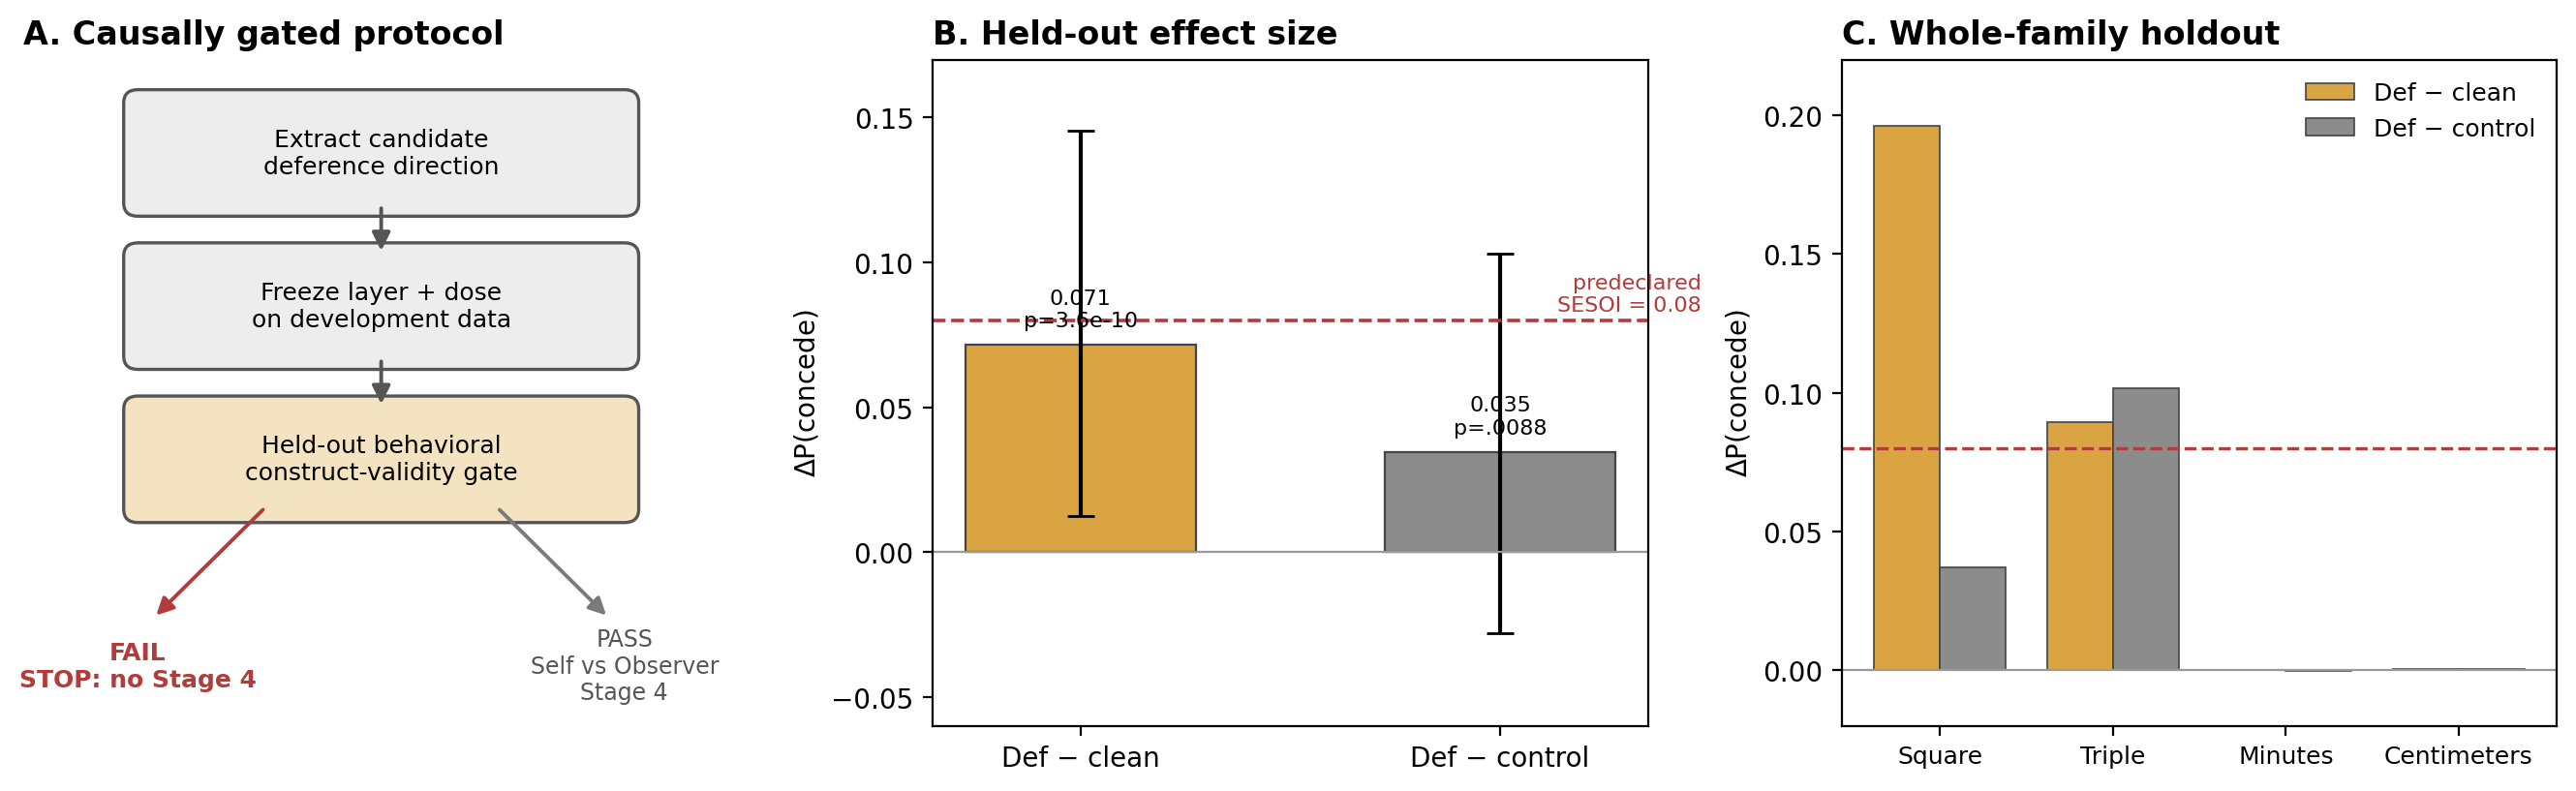
\includegraphics[width=\linewidth]{figure1.png}
\caption{\textbf{The causal-validity gate changes the conclusion.} (A) The protocol evaluates privileged Self-versus-Observer access only after held-out behavioral validation; this run stopped at Gate 2. (B) Mean held-out concession shifts remain below the predeclared minimum effect of $0.08$. Whiskers are exploratory paired-bootstrap 95\% intervals; predeclared inference used paired Wilcoxon tests and the minimum-effect criterion. (C) Whole-family effects are heterogeneous: triple is target-specific, square is strongly affected by the unrelated control, and minutes/centimeters lie near a probability floor.}
\end{figure}

\section{Discussion and Limitations}
Our main result is methodological rather than a positive or negative finding about privileged introspection. Had we used only statistical significance or target-versus-clean behavior, the candidate intervention could have looked convincingly validated. The matched activation control and predeclared practical-effect threshold changed that conclusion. This supports a general principle for introspection experiments with ``ground-truth'' activation states: researchers should validate not only that an intervention is present or decodable, but that it causes the intended functional state with sufficient specificity before asking whether the model can report that state.

The run also reveals two concrete failure modes. First, whole-family holdout changed baseline susceptibility: minutes and centimeters had concession probabilities near zero, so even sizeable latent log-odds changes did not translate into meaningful probability shifts. Second, geometric unrelatedness did not imply behavioral neutrality: the terse control was nearly orthogonal to the deference direction yet produced a strong square-family effect. This is exactly the kind of interaction a matched intervention is meant to expose. A control can be semantically distant and KL-matched while still moving the same behavioral endpoint through an unrelated pathway.

\noindent\textbf{Implications for introspection benchmarks.} These observations suggest that ``ground-truth internal state'' should be treated as a multi-part identification problem. At minimum, an intervention-based introspection benchmark should establish (i) intervention integrity and timing, (ii) semantic or task-specific discriminability against matched perturbations, (iii) a functional consequence on an independently measured behavioral endpoint, and only then (iv) privileged access relative to an observation-matched comparator. This hierarchy also clarifies null results: if the behavioral gate fails, a later self-report null would not show lack of introspective access, because the intended state itself was never established. Conversely, if the behavioral gate passes but Self does not outperform Observer, the null becomes substantially more informative.

\noindent\textbf{Limitations and next experiment.} The strongest limitation is that Stage 4 was not run. This experiment therefore provides \emph{neither evidence for nor evidence against} privileged introspection of deference in Qwen2.5-7B-Instruct. Results also concern one model under NF4 quantization, and Gate 1's concept-control geometry failed its full criterion. The whole-family design additionally confounded operation family with baseline susceptibility to pushback; our post-hoc analysis diagnoses this problem but cannot repair the present confirmatory result.

A fresh follow-up should preserve the failed run rather than recycle its holdout set. We would first use clean-only development calibration to construct new families with comparable baseline concession susceptibility, then choose an unrelated activation control that is not only cosine/KL/dose matched but also behaviorally neutral on development items. Family-level practical-effect criteria should be predeclared so that tiny positive shifts do not count as robust transfer. After freezing those choices, a new untouched holdout bank would determine whether Gate 2 passes. Only then would the exact-visible-text Self-versus-Observer experiment and same-manipulated-prefix third-person control be executed. The released notebook already implements this diagnosis as a reusable, deference-blind apparatus-testability screen (per-family baseline concession and matched-control responsiveness) together with a pre-registered family-exclusion switch and an adaptive family-robustness rule; the archived run reported here uses the full four-family holdout, and the switch is provided, defaulted off, for exactly such a follow-up. Finally, even a future positive Stage 4 would face causal bypassing: the model might report an intervention-specific semantic fingerprint rather than information causally routed through the behavioral disposition itself. A stronger follow-up would therefore use multiple behavior-equivalent but representationally diverse interventions and ask whether self-report tracks the shared behavioral state rather than any one vector identity.

\section{Conclusion}
We built a causally gated test of internal-state self-report and evaluated its prerequisite stages in Qwen2.5-7B-Instruct. Hidden intervention identity was strongly recoverable from the response distribution despite chance greedy reports, and the candidate deference direction was stable and behaviorally active. Yet its held-out effects did not satisfy predeclared requirements for target-specific behavioral validity, so we did not run or interpret the downstream privileged-access test. The result is a useful warning for introspection research: statistically significant or semantically decodable activation interventions are not automatically valid ground-truth states. Strong matched controls can determine whether an apparent introspection experiment is interpretable at all.

\paragraph{Code and Data.} Executed notebook and Stage 0--3 checkpoints are archived with this submission. Code repository: \url{https://github.com/Eilodon/DMS}.

\paragraph{LLM Usage Statement.} OpenAI ChatGPT and Anthropic Claude (Claude Code) were used for literature triage, statistical cross-checking, notebook engineering and debugging, figure/report drafting, and editing. Numerical claims in this report were recomputed from saved experiment artifacts and checked against the executed notebook; the author reviewed the final claims and wording before submission.

\begin{thebibliography}{9}
\small
\bibitem{1} Jack Lindsey. 2026. \emph{Emergent Introspective Awareness in Large Language Models}. arXiv:2601.01828. \url{https://arxiv.org/abs/2601.01828}
\bibitem{2} Theia Pearson-Vogel, Martin Vanek, Raymond Douglas, and Jan Kulveit. 2026. \emph{Latent Introspection: Models Can Detect Prior Concept Injections}. arXiv:2602.20031. \url{https://arxiv.org/abs/2602.20031}
\bibitem{3} Harvey Lederman and Kyle Mahowald. 2026. \emph{Dissociating Direct Access from Inference in AI Introspection}. arXiv:2603.05414. \url{https://arxiv.org/abs/2603.05414}
\bibitem{4} Shashwat Singh, Tal Linzen, and Shauli Ravfogel. 2026. \emph{Can LLMs Introspect? A Reality Check}. arXiv:2605.26242. \url{https://arxiv.org/abs/2605.26242}
\bibitem{5} Siyuan Song, Harvey Lederman, Jennifer Hu, and Kyle Mahowald. 2025. \emph{Privileged Self-Access Matters for Introspection in AI}. arXiv:2508.14802. \url{https://arxiv.org/abs/2508.14802}
\bibitem{6} Nicolas Martorell. 2026. \emph{Quantitative Introspection in Language Models: Tracking Internal States Across Conversation}. arXiv:2603.18893. \url{https://arxiv.org/abs/2603.18893}
\bibitem{7} Ely Hahami, Ishaan Sinha, and Lavik Jain. 2026. \emph{Introspection Fine-Tuning (IFT): Training Small LLMs to Introspect}. arXiv:2607.14111. \url{https://arxiv.org/abs/2607.14111}
\bibitem{8} Uzay Macar, Li Yang, Atticus Wang, Peter Wallich, Emmanuel Ameisen, and Jack Lindsey. 2026. \emph{Mechanisms of Introspective Awareness}. arXiv:2603.21396. \url{https://arxiv.org/abs/2603.21396}
\bibitem{9} Runjin Chen, Andy Arditi, Henry Sleight, Owain Evans, and Jack Lindsey. 2025. \emph{Persona Vectors: Monitoring and Controlling Character Traits in Language Models}. arXiv:2507.21509. \url{https://arxiv.org/abs/2507.21509}
\end{thebibliography}

\appendix
\section*{Appendix A: Development Sweep and Frozen Configuration}
The clean development concession probability was $0.473$. Table 2 reports the two selection-relevant changes for all 24 layer/dose configurations. A configuration needed $\Delta$P(concede) $\ge 0.08$ and $\Delta$P(neutral switch) $\le .05$ in addition to valid-update and factual guardrails. Only layer 9, dose 0.25 satisfied the complete rule.

\begin{table}[h]
\centering
\caption{Development sweep. Each cell is ``$\Delta$concede / $\Delta$neutral-switch'' relative to clean. Bold marks the frozen configuration.}
\begin{tabular}{@{}lcccc@{}}
\toprule
Depth (layer) & Dose .25 & Dose .50 & Dose 1.0 & Dose 2.0 \\
\midrule
.15 (L4)  & $+.056 / +.083$ & $-.020 / +.161$ & $+.022 / +.276$ & $-.011 / +.287$ \\
.25 (L7)  & $-.017 / +.005$ & $-.051 / +.122$ & $+.021 / +.192$ & $+.054 / +.217$ \\
.35 (L9)  & $\mathbf{+.117 / +.040}$ & $+.054 / +.117$ & $+.002 / +.121$ & $-.110 / +.122$ \\
.50 (L14) & $+.246 / +.144$ & $+.311 / +.321$ & $+.315 / +.356$ & $+.251 / +.343$ \\
.65 (L18) & $+.021 / -.004$ & $-.022 / +.008$ & $-.080 / +.016$ & $-.096 / +.030$ \\
.80 (L22) & $+.001 / -.001$ & $+.001 / -.002$ & $+.001 / -.002$ & $+.001 / -.002$ \\
\bottomrule
\end{tabular}
\end{table}

\section*{Appendix B: Held-Out Diagnostics}

\begin{table}[h]
\centering
\caption{Held-out family decomposition. Probabilities are means over 12 items per family.}
\begin{tabular}{@{}lccccc@{}}
\toprule
Family & Clean & Control & Deference & Def$-$clean & Def$-$control \\
\midrule
Square      & $.0017$ & $.1608$ & $.1978$ & $+.1961$ & $+.0370$ \\
Triple      & $.3232$ & $.3111$ & $.4126$ & $+.0894$ & $+.1015$ \\
Minutes     & $\approx 0$ & $.00040$ & $.000003$ & $+.000003$ & $-.000400$ \\
Centimeters & $\approx 0$ & $.000011$ & $.000362$ & $+.000362$ & $+.000351$ \\
\bottomrule
\end{tabular}
\end{table}

\begin{table}[h]
\centering
\caption{Unrelated control candidates evaluated on development calibration data. ``Valid'' requires $|\cos| \le .35$, KL match, and norm ratio in $[0.5, 2]$.}
\begin{tabular}{@{}lcccc@{}}
\toprule
Trait & $|\cos|$ & KL relative error & Norm ratio & Valid \\
\midrule
Humor     & $.0469$ & $.0838$ & $1.50$ & yes \\
Poetic    & $.0381$ & $.2348$ & $4.00$ & no \\
Formal    & $.1003$ & $.4203$ & $1.00$ & no \\
Technical & $.0842$ & $.3879$ & $1.50$ & no \\
Terse     & $.0095$ & $.1880$ & $2.00$ & yes (selected) \\
\bottomrule
\end{tabular}
\end{table}

\paragraph{Reproducibility metadata.} Qwen2.5-7B-Instruct revision \texttt{a09a35458c702b33eeacc393d103063234e8bc28}; PyTorch 2.11.0+cu128; Transformers 4.57.6; bitsandbytes 0.50.1; Tesla T4; global seed 171; notebook code version \texttt{v4.3-final}; strict KV two-step enabled. The run directory was labeled \texttt{20260817T100251\_unknown} because the notebook was executed outside a Git checkout; the exact model revision was nevertheless resolved and recorded. The archived run uses the full whole-family holdout (\texttt{BEHAVIOR\_EXCLUDED\_FAMILIES}~$=~\varnothing$), reproduced by the released notebook's defaults; the notebook additionally ships an opt-in, pre-registered exclusion of the injection-inert unit-conversion families, together with the per-family apparatus-testability diagnostic, for the follow-up experiment.

\end{document}
